\documentclass{article}

\usepackage{graphicx}
\usepackage{hyperref}
\usepackage{listings}
\usepackage{lmodern}  % for bold teletype font
\usepackage{amsmath}  % for \hookrightarrow
\usepackage{xcolor}   % for \textcolor
\usepackage{biblatex}

\title{Evaluating Performance of Different FIFO Queues in the Java Virtual Machine's Garbage Collector}
\date{2019-03-16}
\author{Guy Ezer ; Ran Hochshtet}

% images path
\graphicspath { {./images/} }

% newline between paragraphs
\usepackage[parfill]{parskip}
\lstset{
  basicstyle=\ttfamily,
  columns=fullflexible,
  frame=single,
  breaklines=true,
  postbreak=\mbox{\textcolor{red}{$\hookrightarrow$}\space},
}

\begin{document}
  \maketitle

  \newpage

  \section{Intro}
  \subsection{Abstract}
  \paragraph
  Large-scale multicore architectures create new challenges for garbage collectors. 
  The paper \href{https://hal.inria.fr/hal-00868012/document}{``A study of the scalability of stop-the-world garbage collectors on multicores``} analyzed the HostSpot JVM`s garbage collector (GC) called \textbf{Parallel Scavenge}, identified its bottlenecks and tried to address them using parallel programming techniques - such as using a lock-free task queue - as we saw in class.

  The paper modified the HotSpot JVM to support the proposed changes and compared both the non-modified JVM and the modified JVM on standard benchmarks and showed that the lock-free approach improved the GC throughput.

 Further research can be done on the concurrent FIFO queue in the GC context - 
 the concurrent FIFO queue is a fundamental data structure, and designing efficient concurrent queues has attracted a lot of research attention.
 Today, the best performing queues still have contended hot spots (namely, the queue head and tail). These hot spots are particularly painful when queues are used on modern non-uniform memory access (NUMA) machines. These machines have multiple processors, each of which has multiple cores.
 The overhead of contended hot spots on a NUMA machine is very high because of the latency of transferring a cache line between processors is orders of magnitudes higher than transferring a line between cores in the same processor.

 In our work, focused on the parallel task queue and study the impact of using different concurrent queues as the GC scheduling queue on the GC itself and the application on NUMA systems.

 We used an existing queue project that was provided by adam, which contains the implementation of two lock-free queues: \textit{HLCRQ} and \textit{MS-QUEUE}. With the following numa-transformations:
 \begin{itemize}
   \item \textbf{Simple Schedualing}
   \item \textbf{Reference Counting}
   \item \textbf{Cache Miss Sensing}
   \item \textbf{Workload Adaptive Transformation}
 \end{itemize}

 We maintain that library at \texttt{./msqueue-schedualing/}. Further detailed can be found at \textbf{\textit{Integrating the NUMA Aware Queues}}.

 \newpage

 \subsection{Parallel Scavenge}
 \textbf{Parallel Scavenge} is the default GC of OpenJDK’s HotSpot virtual machine and is the one that provides the best performance when the number of cores increases\cite{paper}
 Parallel Scalability is a stop-the-world GC, meaning that the GC pauses the application threads during collection to prevent concurrent memory accesses from the application.

 The garbage collection is activated once the the memory buffers that are provided to the application are full; The following diagram shows the phases of Parallel Scavenge:

 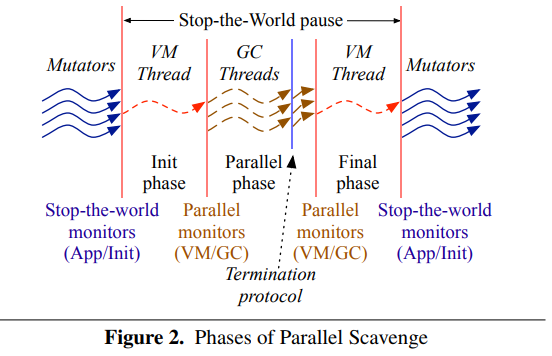
\includegraphics[width=\textwidth]{gc_phases.png}

 During the initialisation phase, a single thread, called the VM thread, prepares GC tasks, which are executed in the parallel phase by the GC threads.
 As soon as all the mutators are suspended, the VM thread initialises the queue of GC tasks. The task queue is implemented as a singly-linked list that is protected by a Monitor.
 Each GC thread fetches tasks from the queue in a concurrent matter. 
 
 The paper showed an improvement in the GC throughput addressing the bottleneck caused by the queue's monitor - by changing the queue to a MS-QUEUE, which is \textbf{lock-free}, performance is improved due to threads not having to wait for the shared lock.

 \newpage

 \section{Integration}
 We had \textit{a LOT} of problems during the compilation of the JVM

 \subsection{Initial Compilation}
 The Initial compilation of the provided version of OpenJDK took several days; We provide a script called \textit{compile.sh} which compiles the whole project.
 
 Since the code is very outdated, a lot of patches had to be made in order for the JDK to be compiled - which includes:
 \begin{itemize}
   \item Changing timestaps of older files - the build engine terminates when it encounters file that are over 10 years "old"
   \item Creating a local HTTP server to host resources that the build engine requires; the original server died:

   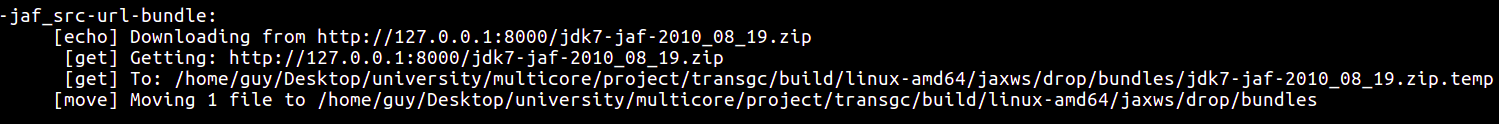
\includegraphics[width=\textwidth]{local_http_server.png}
   \item applying a few patches to libalsa (my distribution's libalsa was too new for the JDK to build on - the API was broken)
 \end{itemize}

 Luckily, we found the \href{http://www.voidcn.com/article/p-zayqisji-va.html}{following blog post} which covered the rest of the unresolved errors.

 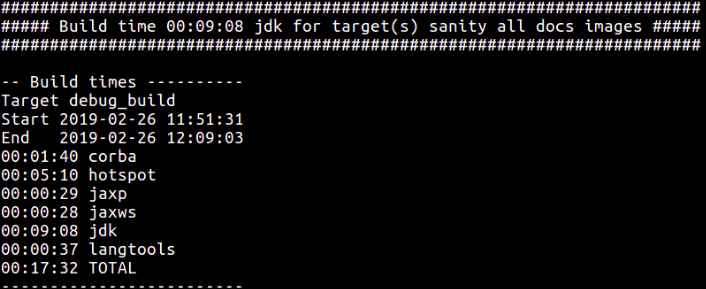
\includegraphics[width=\textwidth]{initial_build.png}

 \newpage

 \subsection{Integrating the NUMA Aware Queues} \label{queues:integration}
 After some thought, we decided that the queues that we want to integrate into the JVM will be linked against it as a \textbf{shared library}. Here are some supporting arguments:
 \begin{itemize}
   \item Hacking the build engine is complicated enough as is - many Makefile are generated and changes has to be made in several files, building as a shared library would probably take us less time.
   \item The queue library was compiled with specific flags and options; Applying those to the queue library could cause unexpected behavior
   \item Compiling the JVM takes quite a while, and some times has to be compiled from scratch. Switching between NUMA transformation will only require to recompile the shared library
 \end{itemize}

 We then proceeded to define an API for the JVM to use:
 \begin{lstlisting}[language=C]
   extern void numa_enqueue(Globals* context, Object arg, int pid);

   extern Object numa_dequeue(Globals* context, int pid);
   
   extern Globals* create_global_context();
 \end{lstlisting}

 We tried to mask out the NUMA transformation method that is beging used and the queue structure from the JVM in order to create a consistant interface. Sadly, we have to re-compile the project when switching between MSQUEUE and HLCRQ because the \textit{Globals} structure contains the inner queue definition.

 \begin{itemize}
   \item The \textit{Globals} is used to save the queue used and the schedualing method that was chosen.
   \item \textit{numa\_enqueue} is used to enqueue an address.
   \item \textit{numa\_dequeue} is used to dequeue an andress from the queue. If the queue is empty - it returns NULL.
 \end{itemize}

 Here is the implementation of the API. It can be seen that \textit{numa\_dequeue} performs a NUMA transformation on the queue's tail and head:

 \begin{lstlisting}[language=C]
   #include "numa_queue.h"
   
   extern void numa_enqueue(Globals* context, Object arg, int pid) {
       enqueue(&context->queue, arg, pid);
   }
   
   extern Object numa_dequeue(Globals* context, int pid){
       Object obj;
   
   #ifdef MSQUEUE
       cluster_scheduler_start_op(&context->atomic_scheduler, &context->queue.Head);
   #else
       cluster_scheduler_start_op(&context->atomic_scheduler, &context->queue.Head->head);
   #endif
       obj = (Object)(dequeue(&context->queue, pid));
   #ifdef MSQUEUE
       cluster_scheduler_end_op(&context->atomic_scheduler, &context->queue.Tail);
   #else
       cluster_scheduler_end_op(&context->atomic_scheduler, &context->queue.Tail->tail);
   #endif
       
       return obj;
   }
   
   extern Globals* create_global_context() {
       Globals* context = (Globals*)malloc(sizeof(Globals));
       SHARED_OBJECT_INIT(&context->queue);
   #ifdef MSQUEUE
       cluster_scheduler_init(&context->atomic_scheduler, &context->queue.Head, &context->queue.Tail);
   #else
       cluster_scheduler_init(&context->atomic_scheduler, &context->queue.Head->head, &context->queue.Tail->tail);
   #endif
       return context;
   }
 \end{lstlisting}

 For future reference, the following places in the JDK`s build system were changed in order to link agains \textit{libnuma\_queue}:
 \begin{itemize}
   \item \texttt{./hotspot/make/linux/build.sh} - Contains the top-level \textit{LD\_LIBRARY\_PATH}.

     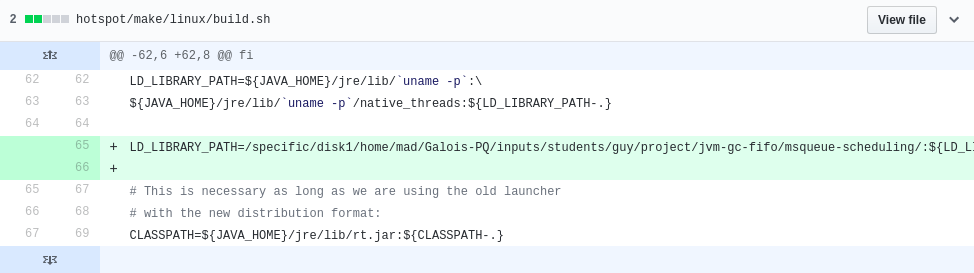
\includegraphics[width=\textwidth]{build.png}
   \item \texttt{./hotspot/make/linux/makefiles/buildtree.make} - Generator of Makefiles for different targets. Generated the Makefile for the Parallel Scavenge implementation.

     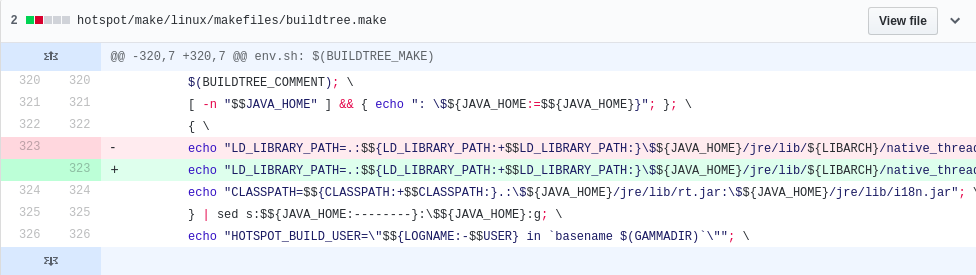
\includegraphics[width=\textwidth]{buildtree.png}
   \item \texttt{./hotspot/make/linux/makefiles/launcher.make} - Makefile for the gamma launcher, which is a required test that is run during the build (if we understood it correctly).

     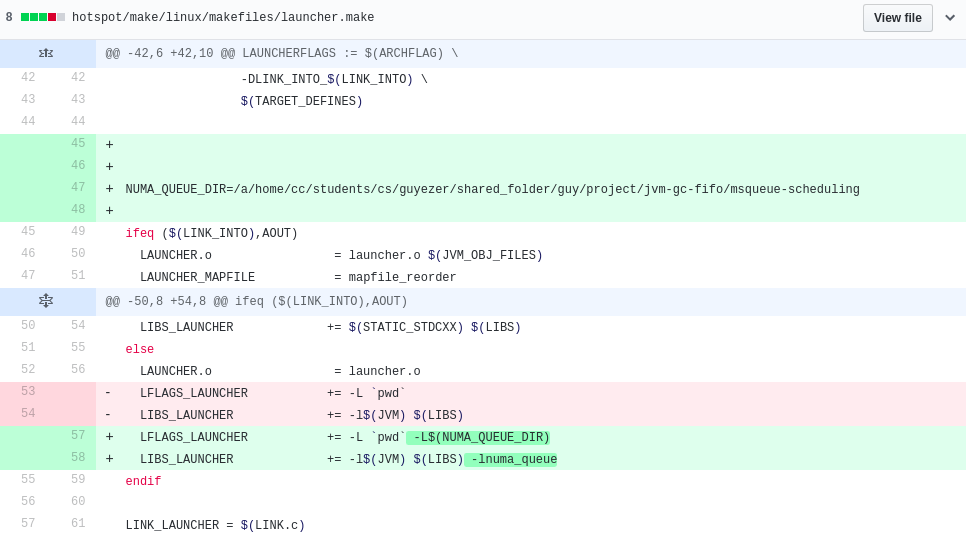
\includegraphics[width=\textwidth]{launcher.png}
 \end{itemize}

 \newpage

 \section{Benchmarks}
 \subsection{Chosen Benchmarks}
 Initially, we wanted to run the same benchmarks that were introduced in the paper, but each came with its own set of problems:

 \begin{itemize}
   \item \textbf{SPECjbb2005} isnt freely available
   \item \textbf{DaCapo} was very unstable. We tried hacking it quite a bit but with not too much success.
   \item \textbf{SPECjvm2008} - which several of its benchmarks were used in the paper. We only used \textit{transform.xml}.
 \end{itemize}

 \subsection{Benchmarks Setup}
 We ran \textit{transform.xml} with an increasing number of cores dedicated for the GC.
 The GC's throughput is evaluated as:
 \begin{equation}
	 \frac{young\_generation\_work}{total\_time\_spent\_in\_gc}
 \end{equation}

 \begin{itemize}
   \item \textit{young generation work} is the total bytes that were transferred in the young generation
   \item \textit{total time spent in gc} is the total execution time in the GC
 \end{itemize}

 Luckily for us, the initial author had already printed these values (and more) in the JVM exit point:

 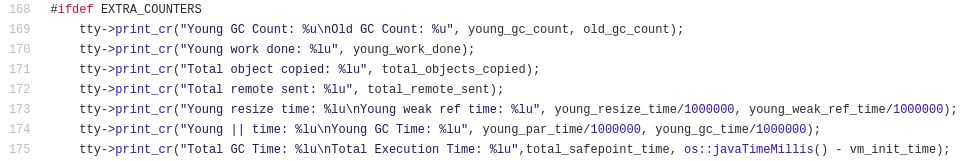
\includegraphics[width=\textwidth]{gc-debug-prints.png}

 The script \texttt{run\_benchmarks.sh} runs the benchmarks with different configurations - it iterates on all the different queues (msqueue and hlcrq), numa schedualing methods and an increasing number of cores. It saves the result to log files which are later on parsed by it into a .csv file - in which its left colomn is the number of processes and its right column is the GC throuhput for the given core.
This gave us the ability to quickly analyze results of different runs.

 \newpage

 \subsection{transform.xml Results}
 Our result were not good - there may have been noise or that we have ran out tests wrogly. Since we couldn't get much run time on the server (after fixing all of our bugs) we did not have time to inspect that.

 \subsubsection{without changes}

 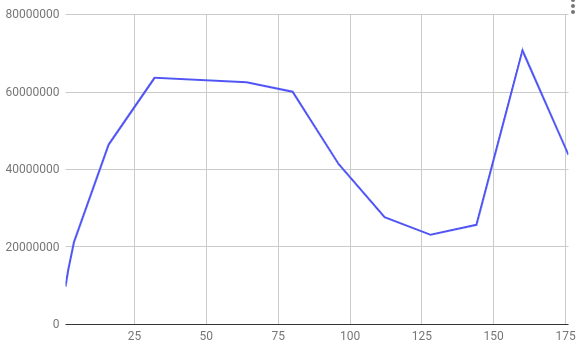
\includegraphics[width=\textwidth]{graph-no-changes.png}

 Here you can see that, generally, that as the number of cores go up, the throughput goes up - until it reaches its peak at 32 cores, and then the throughput goes down. This could be because of contention over a shared resource.
 

 \subsubsection{MSQUEUE}

 \subsubsection{HLCRQ}

 \subsection{Conclusion}

  % references
  \medskip
  \newpage

  \begin{thebibliography}{9}
    \bibitem{paper}
      Lokesh Gidra, Gael Thomas, Julien Sopena and Marc Shapiro: "A Study of the Scalability of Stop-the-world Garbage Collectors on Multicores"
      \\\texttt{https://hal.inria.fr/hal-00868012/document}
  \end{thebibliography}

\end{document}
